\documentclass[
% opciók nélkül: egyoldalas nyomtatás, elektronikus verzió
% twoside,     % kétoldalas nyomtatás
% tocnopagenum,% oldalszámozás a tartalomjegyzék után kezdődik
]{thesis-ekf}
\usepackage[T1]{fontenc}
\PassOptionsToPackage{defaults=hu-min}{magyar.ldf}
\usepackage[magyar]{babel}
\usepackage{mathtools,amssymb,amsthm,pdfpages}
\footnotestyle{rule=fourth}

\newtheorem{tetel}{Tétel}[chapter]
\theoremstyle{definition}
\newtheorem{definicio}[tetel]{Definíció}
\theoremstyle{remark}
\newtheorem{megjegyzes}[tetel]{Megjegyzés}

\begin{document}
\institute{Matematikai és Informatikai Intézet}
\title{Jelenlét követő alkalmazás fejlesztése}
\author{Györkis Tamás\\Programtervező informatikus BSc}
\supervisor{Dr. Király Roland\\Egyetemi docens}
\city{Eger}
\date{2024}
\maketitle
\tableofcontents

\chapter*{Bevezetés}
\addcontentsline{toc}{chapter}{Bevezetés}
Amikor szakdolgozati témaválasztás előtt álltam, sokat gondolkoztam a témán. Mindenképpen egy olyan alkalmazást szerettem volna elkészíteni, mely ténylegesen hasznos is lehet. Egyetemi éveim alatt demonstrátorként tanítottam több féléven át az egyetemen, és innen jött a felismerés, hogy jó lenne, ha a hallgatók jelenlétét, hiányzásait ne táblázatokban kelljen vezetni, hanem egy külön eszköz legyen rá készítve. Innen származik az alkalmazás ötlete.

A megvalósítás során törekedtem arra, hogy egy jól átlátható, ergonomikus weboldalt készítsek, amit -- esetleges kisebb módosításokkal -- ne csak egyetemi környezetben lehessen használni. Ezekből kifolyólag egy webalkalmazást készítettem, mivel ezt a legegyszerűbb elérni, hiszen csak egy webböngésző szükséges hozzá. A tanulók és tanárok által használt oldalak reszponzívan lettek elkészítve, ezáltal biztosítva, hogy mobiltelefonon is használni lehessen. Illetve az alkalmazás PWA funkciókkal rendelkezik, aminek jelentőségére később térek ki, de előjáróban annyit érdemes megemlíteni róla, hogy lehetővé teszi a weboldal alkalmazásként való telepítését számítógép és telefon esetén is, ezáltal egy rendes alkalmazás érzését keltve.

A megvalósításhoz a Laravel keretrendszert használtam, mely egy PHP alapú, MVC keretrendszer, amivel tanulmányaim során találkoztam, és egyből megkedveltem. Nem titkolt célom a szakdolgozatommal, hogy bemutassam, hogy a mai, JavaScript preferált világban, továbbra is lehetséges modern, a mai kort kielégítő weboldalt készíteni PHP segítségével, amihez különböző csomagokat alkalmaztam, amiknek működését, illetve egymással való működését a későbbiekben fogom kifejteni.

\chapter{Alkalmazás bemutatása}
\section{Adatbázis}

\Aref{database} ábrán látható az alkalmazás által használt adatbázis, egyed-kapcsolat diagrammal ábrázolva, melyről szeretnék néhány szót ejteni.

\begin{figure}[ht!]
	\centering
	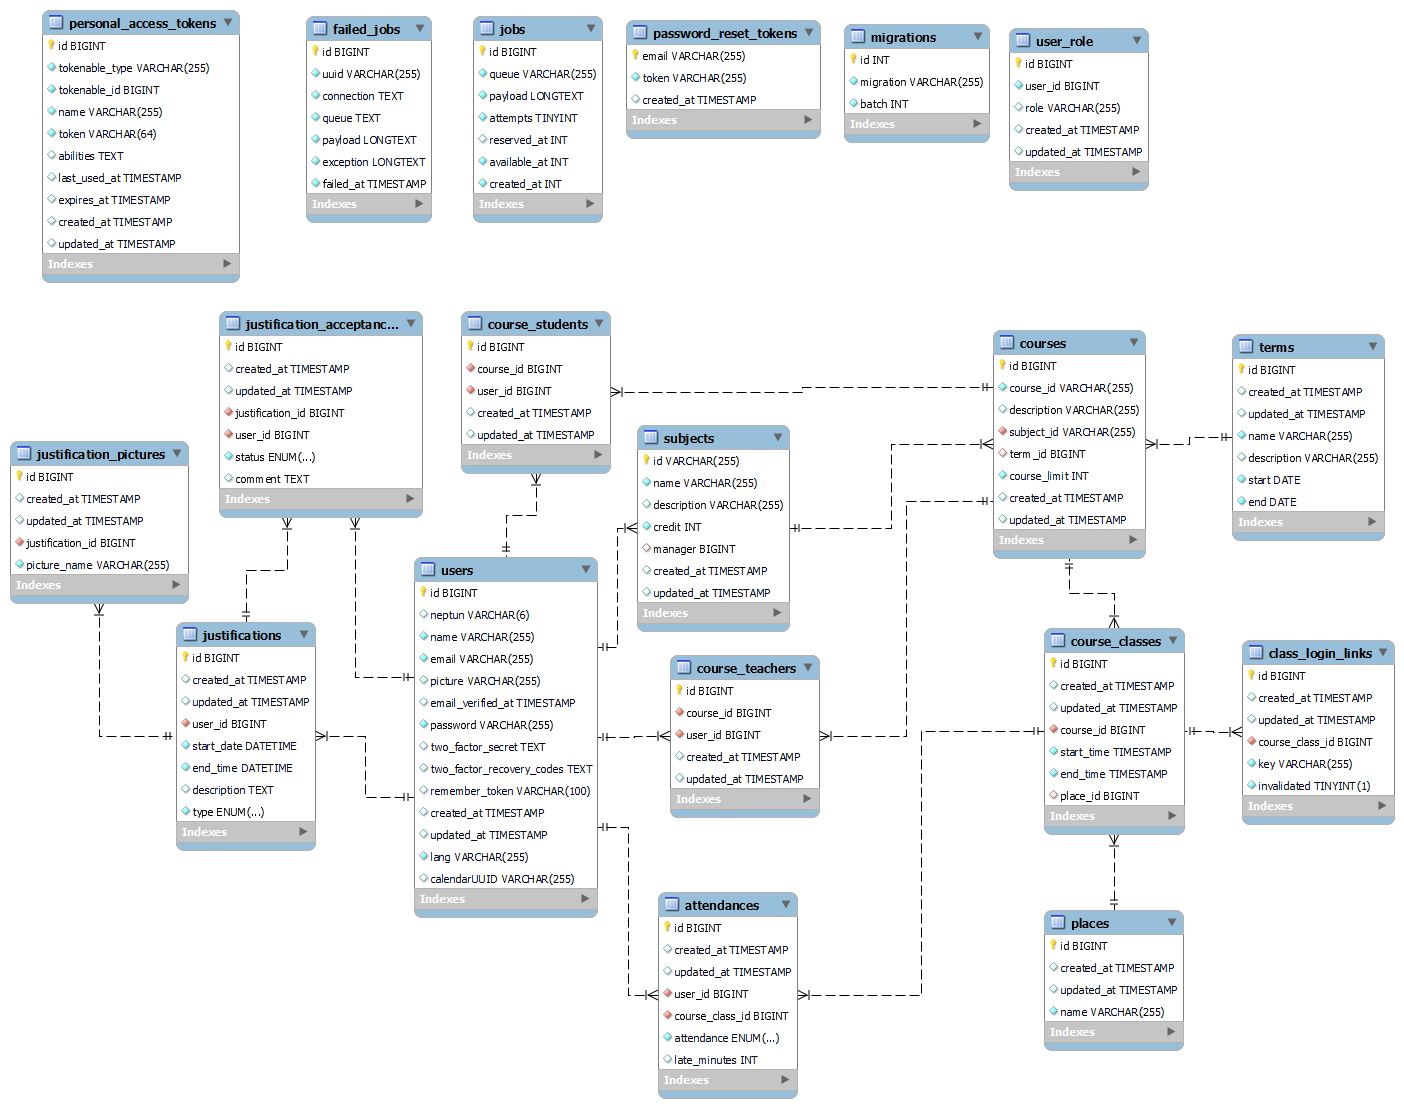
\includegraphics[width=15cm]{../pictures/db.png}
	\caption{Az alkalmazás által használt adatbázis.}
	\label{database}
\end{figure}

\begin{itemize}
	\item \emph{users}: ez a tábla tárolja a felhasználók adatait. Minden felhasználóról tárolunk egy azonosítót, egy Neptun\cite{Neptun} kódot\footnote{A neptun kód egy 6 karakter hosszú, egyedi azonosító.}, nevet, email címet, egy titkosított jelszót, egy profilképet, a felhasználó által használt nyelvet, illetve egy UUID-t, azaz egy egyedi azonosítót, amit az órarend exportálásához lehet használni, erről később. Az azonosító oszlopra azért van szükség, mivel az alkalmazás fel van készítve arra, hogy Neptun kód nélkül rendelkező felhasználókat is tudjon kezelni.
	\item \emph{terms, places}: a félévek és termek (helyek) tárolására szolgáló táblák.
	\item \emph{subjects, courses, course\_classe, class\_login\_links}: ezen táblák tárolják a tantárgyakat (amik többek között rendelkeznek egy azonosítóval, névvel, leírással, kreditértékkel, és egy tantárgyfelelőssel), a tantárgyakhoz tartozó kurzusokat (amihez tárolok egy azonosítót, ami minden esetben egyedi, egy kurzus azonosítót, ami minden félév és tantárgy esetében kell egyedinek lennie, tartozik hozzá egy félév, illetve egy létszám limit), illetve kurzusokhoz pedig órák (amiknek van egy kezdete, vége, illetve egy terem, ahol tartják). Az utolsó tábla pedig az órákhoz tartozó bejelentkező linkeket tartalmazza, ennek jelentőségéről kicsit később.
	\item  \emph{attendances}: itt tárolom az egyes kurzusok résztvevőinek az órai jelenléteit, melyek lehetnek: nincs kitöltve, jelen, késés (mely esetben percben lehet tárolni a mértékét), hiányzás, igazolt hiányzás.
	\item \emph{justification, justification\_acceptances, justification\_pictures}: ezek a táblák tárolják az igazolásokat, az igazoláshoz tartozó feltöltött képeket, illetve az igazolásban érintett tanárok válaszát, hogy elfogadják-e ó, vagy sem.
	\item Az egyéb, nem említett táblák inkább kapcsolótábla funkciót töltenek be, vagy a keretrendszernek vannak rá szükségei. Például a \emph{jobs} tábla a háttérben végrehajtandó feladatokat (job) tartalmazza.
\end{itemize}

Itt érdemes még megemlíteni, hogy a fejlesztés során a MySQL nevezetű, relációs adatbázist használtam, viszont a Laravel keretrendszerből adódóan sok más típusú adatbázis szoftverrel használható az alkalmazás, mivel a táblák felépítése a keretrendszer nyújtotta módon van elkészítve.

\section{Általános információk}

\subsection{Felhasználók}

Az alkalmazás 4 különböző jogkört különböztet meg a felhasználók esetén, melyekből egyszerre többet is birtokolhat a felhasználó:

\begin{itemize}
	\item Szuper adminisztrátor: képes a felhasználók adatainak -- és jogköreinek -- szerkesztésére, illetve az alkalmazás alapbeállításainak módosítására.
	\item Adminisztrátor: a félévek, termek, tantárgyak, kurzusok, órák, készítésére, módosítására, törlésére jogosult.
	\item Tanár: megtekintheti a tanított óráit, kurzusait, hallgatóit. Adminisztrálni tudja az órákon való részvételt, illetve megtekintheti és bírálhatja a hozzá érkezett igazolásokat.
	\item Hallgató: a hozzárendelt óráit, tantárgyait látja, megtekintheti minden kurzus esetén az egyes órák státuszát, illetve igazolásokat hozhat létre
\end{itemize}

Az alkalmazás természetesen rendelkezik bejelentkezés, regisztráció funkciókkal. A felhasználók Neptun\cite{Neptun} kódjuk vagy email címük, illetve a jelszavuk megadásával tudnak bejelentkezni. Regisztrálni csak abban az esetben tudnak, ha az oldal beállításaiban ezt engedélyezték, egyéb esetben a szuper adminisztrátorok tudnak felhasználókat létrehozni vagy importálni. Belépés után  a profil szerkeszthető, a jelszó cserélhető.

\subsection{Általános funkciók}

Bejelentkezés után a főoldalon a felhasználók pár, számukra fontos vagy érdekes információt láthatnak. Tanulók esetében a mai napi óráikat, illetve adminisztrálásra váró igazolásaikat. Tanárok esetén szintén a mai óráikat, illetve a kapott igazolásaikat láthatják. Az adminisztrátorok pár statisztikát láthatnak az oldal kapcsán.

\begin{figure}[ht!]
	\centering
	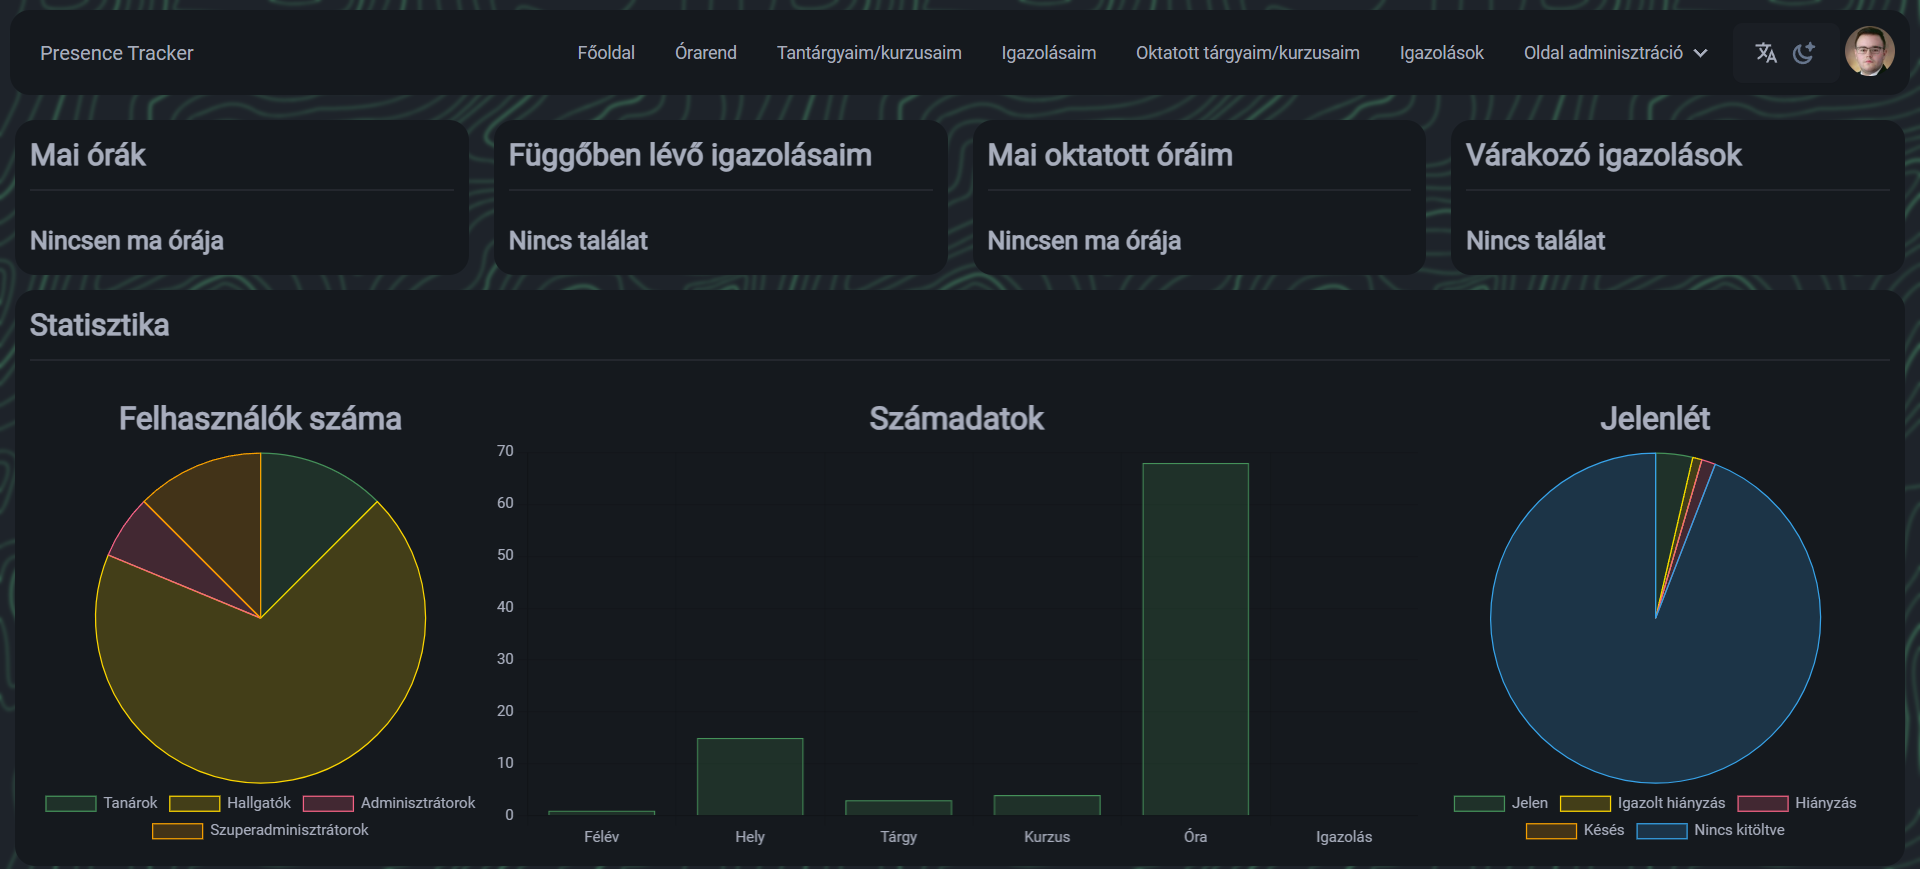
\includegraphics[width=10cm]{../pictures/screenshots/landing.png}
	\caption{A főoldal kinézete abban az esetben, ha a felhasználó minden szerepkörrel rendelkezik. A két bal oldali oszlop a hallgatói nézethez tartozik, a két jobb oldali pedig az oktatóihoz, míg a statisztika adminisztrátorok esetén jelenik meg.}
	\label{landing}
\end{figure}

A profil kép melletti gombra kattintva a felhasználó meg tudja változtatni az oldal nyelvét, Angol és Magyar nyelv közül választva, illetve az oldalt kinézetét: világos és sötét mód között váltogatva. A nyelv beállítása eltárolódik a felhasználóhoz, így újabb bejelentkezés esetén automatikusan beállításra kerül.

Tanuló vagy tanár esetén megjelenik az \emph{Órarend} menüpont is, ahol egy helyen láthatják a heti óráikat a felhasználók. Az egyes órák különböző színekkel jelennek meg, ezzel jelezve, hogy az adott órát a felhasználó tanítja-e, vagy hallgató esetén az órán jelen volt, hiányzott, késett, igazoltan hiányzott, vagy még nincs kitöltve a jelenlét. Lehetőség van az órarend exportálásra is, mely során egy \emph{.ics} kiterjesztésű fájl áll elő. Ez egy széles körben használt általános naptár formátum, amit a felhasználók be tudnak importálni a gyakorian használt naptár programokba\cite{ICS}. Ezáltal kedvenc naptár alkalmazásukban is nyomon tudják követni óráikat.

Lehetőség van a weboldalt alkalmazásként telepíteni, ahogy az \aref{install} ábrán is látható, így gyorsan hozzáférhetnek az alkalmazás funkcióihoz, egy ,,rendes'' alkalmazás érzését keltve ezzel. Ezt a PWA\footnote{Jelentése: Progressive Web App: egy olyan alkalmazás, ami webes technológiákat használ, de platform specifikus alkalmazásként viselkedik.\cite{PWA}} teszi lehetővé, melynek működésére későbbiekben térek ki.

\begin{figure}[ht!]
	\centering
	
\includegraphics[width=8cm]{../pictures/screenshots/install.png}
	\caption{Az oldal telepítésére szolgáló felugró ablak.}
	\label{install}
\end{figure}

\section{Adminisztrátori nézet, funkciók}

\subsection{Felhasználók kezelése}

Szuper adminisztrátor esetén a felhasználó képes kezelni az alkalmazásban tárolt felhasználókat, kivéve saját magát (személyes adatait továbbra is meg tudja változtatni). A listában képes szűrni a felhasználók között, megváltoztatni profil adataikat, jelszavukat alaphelyzetbe állítani, szerkeszteni jogosultsági szintjeiket, illetve akár törölni is őket, ha szükséges. Tud új felhasználókat létrehozni, illetve képes fájlból is importálni adatokat.

\subsection{Alkalmazás konfiguráció}

Szintén a szuper adminisztrátor körébe tartozik az oldal beállításainak kezelése. Az alábbi beállításokat tudja kezelni:
\begin{itemize}
	\item Oldal neve: az oldalon megjelenő név megváltoztatása.
	\item Regisztráció engedélyezése: ezzel lehet engedélyezni, hogy a felhasználók maguktól is tudjanak-e felhasználói fiókot készíteni az oldalon.
	\item Saját Neptun\cite{Neptun} kód megváltoztatása: beállítható, hogy a felhasználó meg tudja magának változtatni ezt az értéket, vagy sem.
	\item Kötelező Neptun kód: az oldal használható ezen kód megadása nélkül is, ez itt szabályozható.
	\item Alkalmazás képe: itt tölthető fel új kép, ami a fő oldalon jelenik meg látogatók esetén.
\end{itemize}

\subsection{Félévek, termek, tantárgyak, kurzusok, órák kezelése}

Minden adminisztrátor képes ezen adatok kezelésére.

Félévek esetén egy nevet, illetve egy kezdő és vég dátumot szükséges megadni. Ellenőrizve van, hogy a félévek nem ütközhetnek egymással. A listában egy pipa jelzi a jelenlegi félévet, ha van ilyen.

A termeknél elegendő egy nevet megadni, ezeket lehet az egyes órákhoz hozzárendelni.

Tantárgyak esetén egy tárgy kódot, egy nevet, egy opcionális leírást, egy kredit értékéket, illetve egy tantárgyfelelőst tárol, akinek rálátása van a tárgy összes kurzusára. Ezen belül minden kurzus egy tárgyhoz kapcsolódik. Ezek szintén rendelkeznek egy kóddal, ami minden tárgy és félév esetén egyedi, szintén egy opcionális leírással, illetve nulla, egy, vagy több tanárral. Minden kurzus egy félévhez van rendelve. A kurzusokhoz hozzárendelhetők a hallgatók, és csak hallgatók.

A kurzusokhoz órák hozhatóak létre, amik a féléven belül lehetnek. Minden óra külön kezdés és vég időponttal rendelkezik, illetve egy teremmel, ahol tartják. Az óra létrehozásakor lehetőség van arra is, hogy a félév végig heti ismétléssel hozza létre az órákat -- természetesen később egyenként lehet őket szerkeszteni, törölni --, ezáltal megkönnyítve az adminisztrációt.

\begin{figure}[ht!]
	\centering
	
\includegraphics[width=15cm]{../pictures/screenshots/newclass.png}
	\caption{Új óra hozzáadása.}
	\label{newclass}
\end{figure}


\section{Tanári nézet, funkciók}
\section{Hallgatói nézet, funkciók}

\chapter{Felhasznált technológiák, csomagok}

\section{Laravel}
\subsection{Keretrendszer alapjai}
\subsection{MVC architektúra}
\subsection{Eloquent ORM}
\subsection{Blade templating engine}
\subsection{Laravel Fortify}
\subsection{Események, queue}
\subsection{Email küldés}

\section{Tailwind}
\subsection{DaisyUI}

\section{LiveWire}
\subsection{Ismertető, a csomag működése}
\subsection{LiveWire és SPA}
\subsection{Komponensek és data binding}
\subsection{Események, lapozás}
\subsection{Alpine.js: LiveWire és JavaScript kapcsolata}
\subsection{WireToast: LiveWire alapú értesítések}

\section{Websocket és Pusher szerviz}
\subsection{Websocket jelentősége}
\subsection{Pusher}
\subsection{Websocket integrálása a keretrendszerbe}
\subsection{Csatornák, események létrehozása}
\subsection{Események fogadása JavaScript, LiveWire esetén}

\section{QR-kód generálás}

\section{Naptár - FullCalendar.js}
\subsection{Beállításai}
\subsection{Kapcsolat a keretrendszerrel LiveWire segítségével}

\section{Diagramok - Chart.js}
\subsection{Beállításai}
\subsection{Kapcsolat a keretrendszerrel LiveWire segítségével}

\section{Progressive Web Apps}
\subsection{A PWA jelentése, jelentősége}
\subsection{Laravel PWA csomag}
\subsection{A manifest fájl}
\subsection{Service Worker}

\chapter{Az alkalmazás tesztelése}
\section{Manuális tesztelés}
\section{Automatizált tesztelés}
\section{Terheléses tesztelés}
\section{Laravel Pint és Github actions}

\chapter{Alkalmazás telepítése}
Az alkalmazás a szakdolgozat védés, illetve a záróvizsga időszak alatt elérhető a \url{https://szakdolgozat.ddns.net} címen, ahol ki lehet próbálni az alkalmazást. Pár alapértelmezett felhasználó elérhető:
\begin{itemize}
	\item Szuper adminisztrátor:
	\begin{itemize}
		\item Felhasználónév: \emph{SADMIN}
		\item Jelszó: \emph{superadmin}
	\end{itemize}
	\item Adminisztrátor:
	\begin{itemize}
		\item Felhasználónév: \emph{ADMIN0}
		\item Jelszó: \emph{admin}
	\end{itemize}
	\item Tanár:
	\begin{itemize}
		\item Felhasználónév: \emph{TEACHE}
		\item Jelszó: \emph{teacher}
	\end{itemize}
	\item Hallgató:
	\begin{itemize}
		\item Felhasználónév: \emph{STUDEN}
		\item Jelszó: \emph{student}
	\end{itemize}
\end{itemize}
\section{Laravel Forge}
\section{Kézi telepítés lépései}

\chapter*{Összegzés}
\addcontentsline{toc}{chapter}{Összegzés}

\begin{thebibliography}{2}
\addcontentsline{toc}{chapter}{\bibname}

\bibitem{Neptun}
\textsc{SDA Informatika Zrt:} \emph{Neptun alkalmazás leírása}
\\
\url{https://sdainformatika.hu/termekek}, Megtekintés dátuma: 2024.03.21.

\bibitem{ICS}
\textsc{FileInfo.com}: \emph{ICS fájl leírása.}
\\
\url{https://fileinfo.com/extension/ics}, Megtekintés dátuma: 2024.03.21.

\bibitem{PWA}
\textsc{MDN web docs}: \emph{Progressive web apps}
\\
\url{https://developer.mozilla.org/en-US/docs/Web/Progressive_web_apps}, Megtekintés dátuma: 2024.03.21.

\end{thebibliography}

%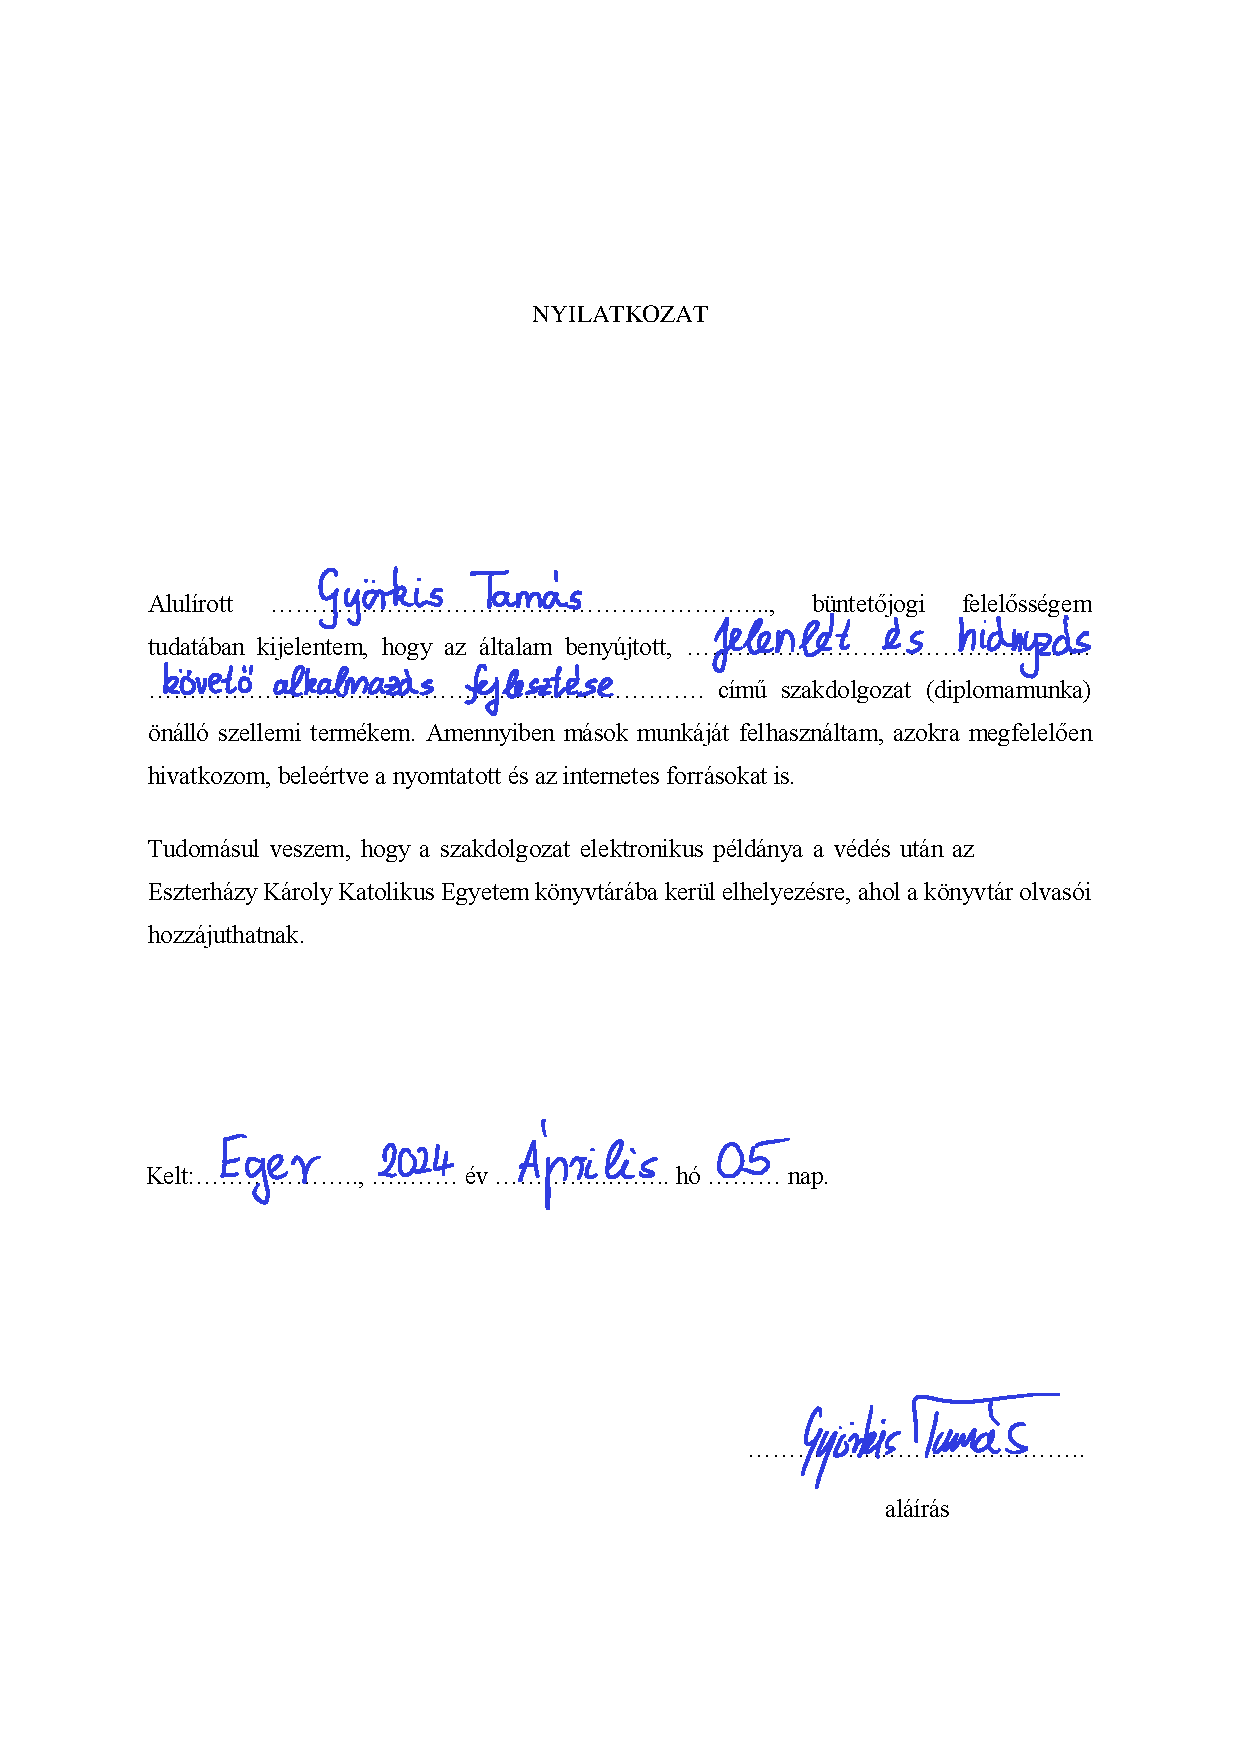
\includepdf{nyilatkozat.pdf}
\end{document}